\documentclass[12pt]{article}
\usepackage{amsmath} % flere matematikkommandoer
\usepackage{amssymb}
\usepackage[utf8]{inputenc} % æøå
\usepackage[T1]{fontenc} % mere æøå
\usepackage[danish]{babel} % orddeling
\usepackage{listings}
\usepackage{color}
\usepackage{enumerate}
\usepackage{algpseudocode}
\usepackage{algorithm}
\usepackage{mathtools}
\definecolor{dkgreen}{rgb}{0,0.6,0}
\definecolor{gray}{rgb}{0.5,0.5,0.5}
\definecolor{mauve}{rgb}{0.58,0,0.82}
\DeclarePairedDelimiter\ceil{\lceil}{\rceil}
\DeclarePairedDelimiter\floor{\lfloor}{\rfloor}
 
\lstset{frame=tb,
 language=Java,
 aboveskip=3mm,
 belowskip=3mm,
 showstringspaces=false,
 columns=flexible,
 basicstyle={\small\ttfamily},
 numbers=none,
 numberstyle=\tiny\color{gray},
 keywordstyle=\color{blue},
 commentstyle=\color{dkgreen},
 stringstyle=\color{mauve},
 breaklines=true,
 breakatwhitespace=true
 tabsize=3
}
 
\newcommand{\abs}[1]{\lvert#1\rvert}
\newcommand{\norm}[1]{\lVert#1\rVert}
 
\newenvironment{amatrix}[1]{%
  \left(\begin{array}{@{}*{#1}{c}|c@{}}
}{%
  \end{array}\right)
}
 
{\setlength{\parindent}{0 cm}
 
\title{Test cases - OOSD}
\author{Simon Warg BCS315}
 
\begin{document}
\maketitle

\section*{Usability test}
I følge af god produktudvikling kommer vi at lave nogle usability tests sammen med en test brugere, \textbf{User}. \textbf{User} har idag allerede en hjemmeside hos an anden leverandør end Surftown men ser ikke sig selv som en erfaren brugere. Derfor synes gruppen at han er en passende testere.

Målet med testerne er at finde fejl som viser på forskellige opførsel end det som er forventet ud fra de specificerede resultater i use casen. Der vil også vides hvis programmet leder til nogen fejlagtig stadie hvor kritiske fejl kan opstå.

Fra \textit{Object-Oriented Software Engineering Using UML, Patterns, and JAVA, 3rd edition, 2010, kapitel 11[?]} er der beskrevet at  iden med et usability test ikke er at vise at programmet ikke indeholder nogle felj eller bugs. Iden er at, på en forberedende måde, prøve at finde erhver fejl, design flaws og andre forkerte ting, som vi udviklere har gået miste om, inden programmet gives ud til slutanvenderen. Dette er en god måde at sikkerstille programmets pålidelighed for slutbrugeren og minimerer antalet af fejlagtige stadier i programmet.
 
\subsection*{Usability test med papir}
Da vi i tilfælde ikke har implementeret en password recovery feature så vil følgene test forigå vha. papir.

	\rule{430pt}{1.0pt}
	\makebox[100pt][l]{\textbf{Mål med testet}}
	\makebox[100pt][l]{\parbox{\textwidth}{At \textbf{User} kan nullstille sitt password}}\\
	\rule{430pt}{0.4pt}
	\makebox[100pt][l]{\parbox{80pt}{\textbf{Deltagende aktøre}}}
	\makebox[100pt][l]{\parbox{\textwidth}{\textbf{User} og nogle stykke \textbf{skærmpapir} med printet skærmafbillede}}\\
	\rule{430pt}{0.4pt}
	\makebox[100pt][l]{\parbox{80pt}{\vspace{-200pt}\textbf{Event flow}}}
	\makebox[100pt][l]{\parbox{320pt}{
	\begin{enumerate}
	  \item{\textbf{User} bliver, før testen starter, fortalt at han/hun hånterer sine domæner og web hosting hos Surftowns kontrolpanel. Nu skal han/hun bruge appen til at nullstille sitt password}
	  \item {Foran \textbf{User} bliver det fremlagt den første \textbf{skærmpapir} der forestiller login-skærmen hvor der findes en glemt-password knapp.}
	  \item{Hvis \textbf{User} trykker på et interaktivt område i billedet så vil test managern skifte \textbf{skærmpapir} til den tilsvarende skærmbillede. }
	  \item{Testet afsluttes når \textbf{User} har opnået målet eller hvis \textbf{User} ikke kommer videre til målet.}
	  
	\end{enumerate}
	}}\\

\subsection*{Usability test med iOS Simulatorn}
	\rule{430pt}{1.0pt}
	\makebox[100pt][l]{\textbf{Mål med testet}}
	\makebox[100pt][l]{\parbox{\textwidth}{At \textbf{User} kan logge ind \\ At \textbf{User} kan finde sine hosting services
							\\ At \textbf{User} kan finde sine registrerede domæner}}\\
	\rule{430pt}{0.4pt}
	\makebox[100pt][l]{\parbox{80pt}{\textbf{Deltagende aktøre}}}
	\makebox[100pt][l]{\parbox{\textwidth}{\textbf{User} og en laptop der kører en iOS simulator}}\\
	\rule{430pt}{0.4pt}
	\makebox[100pt][l]{\parbox{80pt}{\vspace{-200pt}\textbf{Event flow}}}
	\makebox[100pt][l]{\parbox{320pt}{
	\begin{enumerate}
	  \item{\textbf{User} bliver, før testen starter, fortalt at han/hun hånterer sine domæner og web hosting hos Surftowns kontrolpanel. Nu skal han/hun logge på og tjekke hvad han/hun haver.}
	  \item {Foran \textbf{User} bliver findes laptopen med simulatorn opstarted og login-skærmen initieret.}
	  \item{Vha. touchpaden på laptopen kan \textbf{User} navigere og interagere med appen.}
	  \item{Testet afsluttes når \textbf{User} har opnået målet eller hvis \textbf{User} ikke kommer videre til målet.}
	  
	\end{enumerate}
	}}\\
	
\subsection*{Resultat}
Brugeren blev informeret om sin rolle og sine mål som han skulle opnå ved at bruge appen.\\
	\rule{430pt}{1.0pt}
	\makebox[100pt][l]{\textbf{Logge ind:}}
	\makebox[100pt][l]{\parbox{\textwidth}{Brugern tastet in brugernavn og password og klikket på "Login" \\ knappen.
									Der var ikke nogle felj der opstået.}}\\
	\rule{430pt}{0.4pt}
	\makebox[100pt][l]{\textbf{Finde services:}}
	\makebox[100pt][l]{\parbox{\textwidth}{Brugern klikket på "Services" fra hoved menyn. Han blevet spurgt \\ hvor mange services han kunne se. Det første svar vi fikk, var et \\ spørgsmål hvor han spurgte hvad type af service han skulle vælge. \\ Bagefter blevet det klart for \textbf{Users} at det var 3 services som \\ var listet på skærmen.}}

	\rule{430pt}{0.4pt}
	\makebox[100pt][l]{\textbf{Finde domains:}}
	\makebox[100pt][l]{\parbox{\textwidth}{Brugern klikket på "Home" fra den nuvarande "Service" og bagefter \\ klikket på "Domains" fra hovedmenyn. Han blevet spurgt hvor mange \\ domæner han kunne se. Han kunne se 3 domæner, hvilket var korrekt. \\ Bagefter minnet vi \textbf{User} at der burdes findes flere domæner på sit \\ konti og spurgte hvad \textbf{User} så vil gøre for at finde dem? Det tog \\ et klikk tilbage til hovedmenyn og så ind i "Domains" igen før \\\textbf{User} optaget at man kunne scrolle, hvor man så kunne finde de\\  resterende domæner.}}
	
\newpage
	\rule{430pt}{0.4pt}
	\makebox[100pt][l]{\textbf{Password reset:}}
	\makebox[100pt][l]{\parbox{\textwidth}{\textbf{User} klikket på "Forgot password" ved login-skærmen, hvorefter et nyt stykke papir fremlades på bordet. \textbf{User} tastet ind sin e-mail og klikket på "Send". Her opstå ikke et felj stadie.}}
	
\begin{figure}
	\centering
	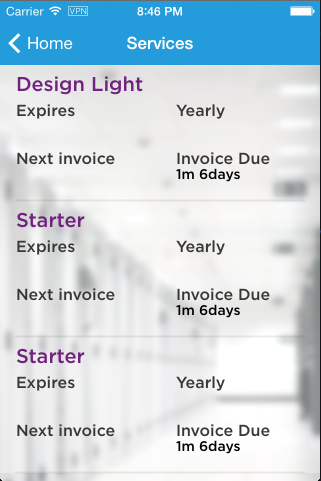
\includegraphics[width=9cm]{ios/services.png}
	\caption{Figuren viser det skærmbilliede test brugeren såg da han klikket på "Services"}
	\label{fig:Services}
\end{figure}

\end{document}
